\documentclass[conference]{IEEEtran}
\IEEEoverridecommandlockouts
% The preceding line is only needed to identify funding in the first footnote. If that is unneeded, please comment it out.
\usepackage{cite}
\usepackage{amsmath,amssymb,amsfonts}
\usepackage{algorithmic}
\usepackage{graphicx}
\usepackage{textcomp}
\usepackage{dsfont}
\usepackage{xcolor}
\usepackage[utf8]{inputenc}
\usepackage{url}
\usepackage{float}
\usepackage[export]{adjustbox}
\def\BibTeX{{\rm B\kern-.05em{\sc i\kern-.025em b}\kern-.08em
    T\kern-.1667em\lower.7ex\hbox{E}\kern-.125emX}}
\begin{document}

\title{Very Small Size Robot Team Strategy\\
}

\author{\IEEEauthorblockN{1\textsuperscript{st} Igor Mourão Ribeiro}
\IEEEauthorblockA{\textit{Computer Engineering Departament} \\
\textit{Instituto Tecnológico de Aeronáutica}\\
São José dos Campos, Brazil \\
igormr98mr@gmail.com}
\and
\IEEEauthorblockN{2\textsuperscript{nd} Paulo Marcelo Tasinaffo}
\IEEEauthorblockA{\textit{Computer Engineering Departament} \\
\textit{Instituto Tecnológico de Aeronáutica}\\
São José dos Campos, Brazil \\
tasinaffo@ita.br}
\and
\IEEEauthorblockN{3\textsuperscript{rd} Marcos Ricardo O. A. Máximo}
\IEEEauthorblockA{\textit{Computer Engineering Departament} \\
\textit{Instituto Tecnológico de Aeronáutica}\\
São José dos Campos, Brazil \\
maximo.marcos@gmail.com}
}

\maketitle


\begin{abstract}
The development of a robust and consistent strategy for a complete team of soccer in the category "Very Small Size" is fundamental to win the matches. After a research phase, it was decided to use the Behavior Tree method for making team decisions. Then, chosen three roles for the players: goalkeeper, main and assistant. Afterwards, a behavior tree for each of them, as well as a technician responsible for ensuring dynamic exchange of roles. The criterion used to evaluate the algorithm was its performance in simulated matches and in national competitions.
\end{abstract}

\begin{IEEEkeywords}
robotics, strategy, decision making
\end{IEEEkeywords}

\section{Introduction}

In the context of robot football, decision-making poses many challenges. The strategy consists of the implementation of an algorithm that is able to use the robot's trajectory planning in the best possible way. This brings us to a higher level of abstraction challenge: deciding what the best decision each robot can take at a certain time considering limitations of possible trajectories to be followed.

In this project, we worked with the robots of the IEEE Very Small Size (VSS) competition: a fully automated robot soccer competition in which each robot has a maximum size of 7.5 cm cube. The football field is 1.5 m long and 1.3 m wide. Each team has 3 players: they can take dynamic positions, as goalkeeper and striker, during a game. A camera provides the aerial view with the positions of all elements of the match. The complete rules can be read in \cite{CBR2008}.

\begin{figure}[H]
	\centering
	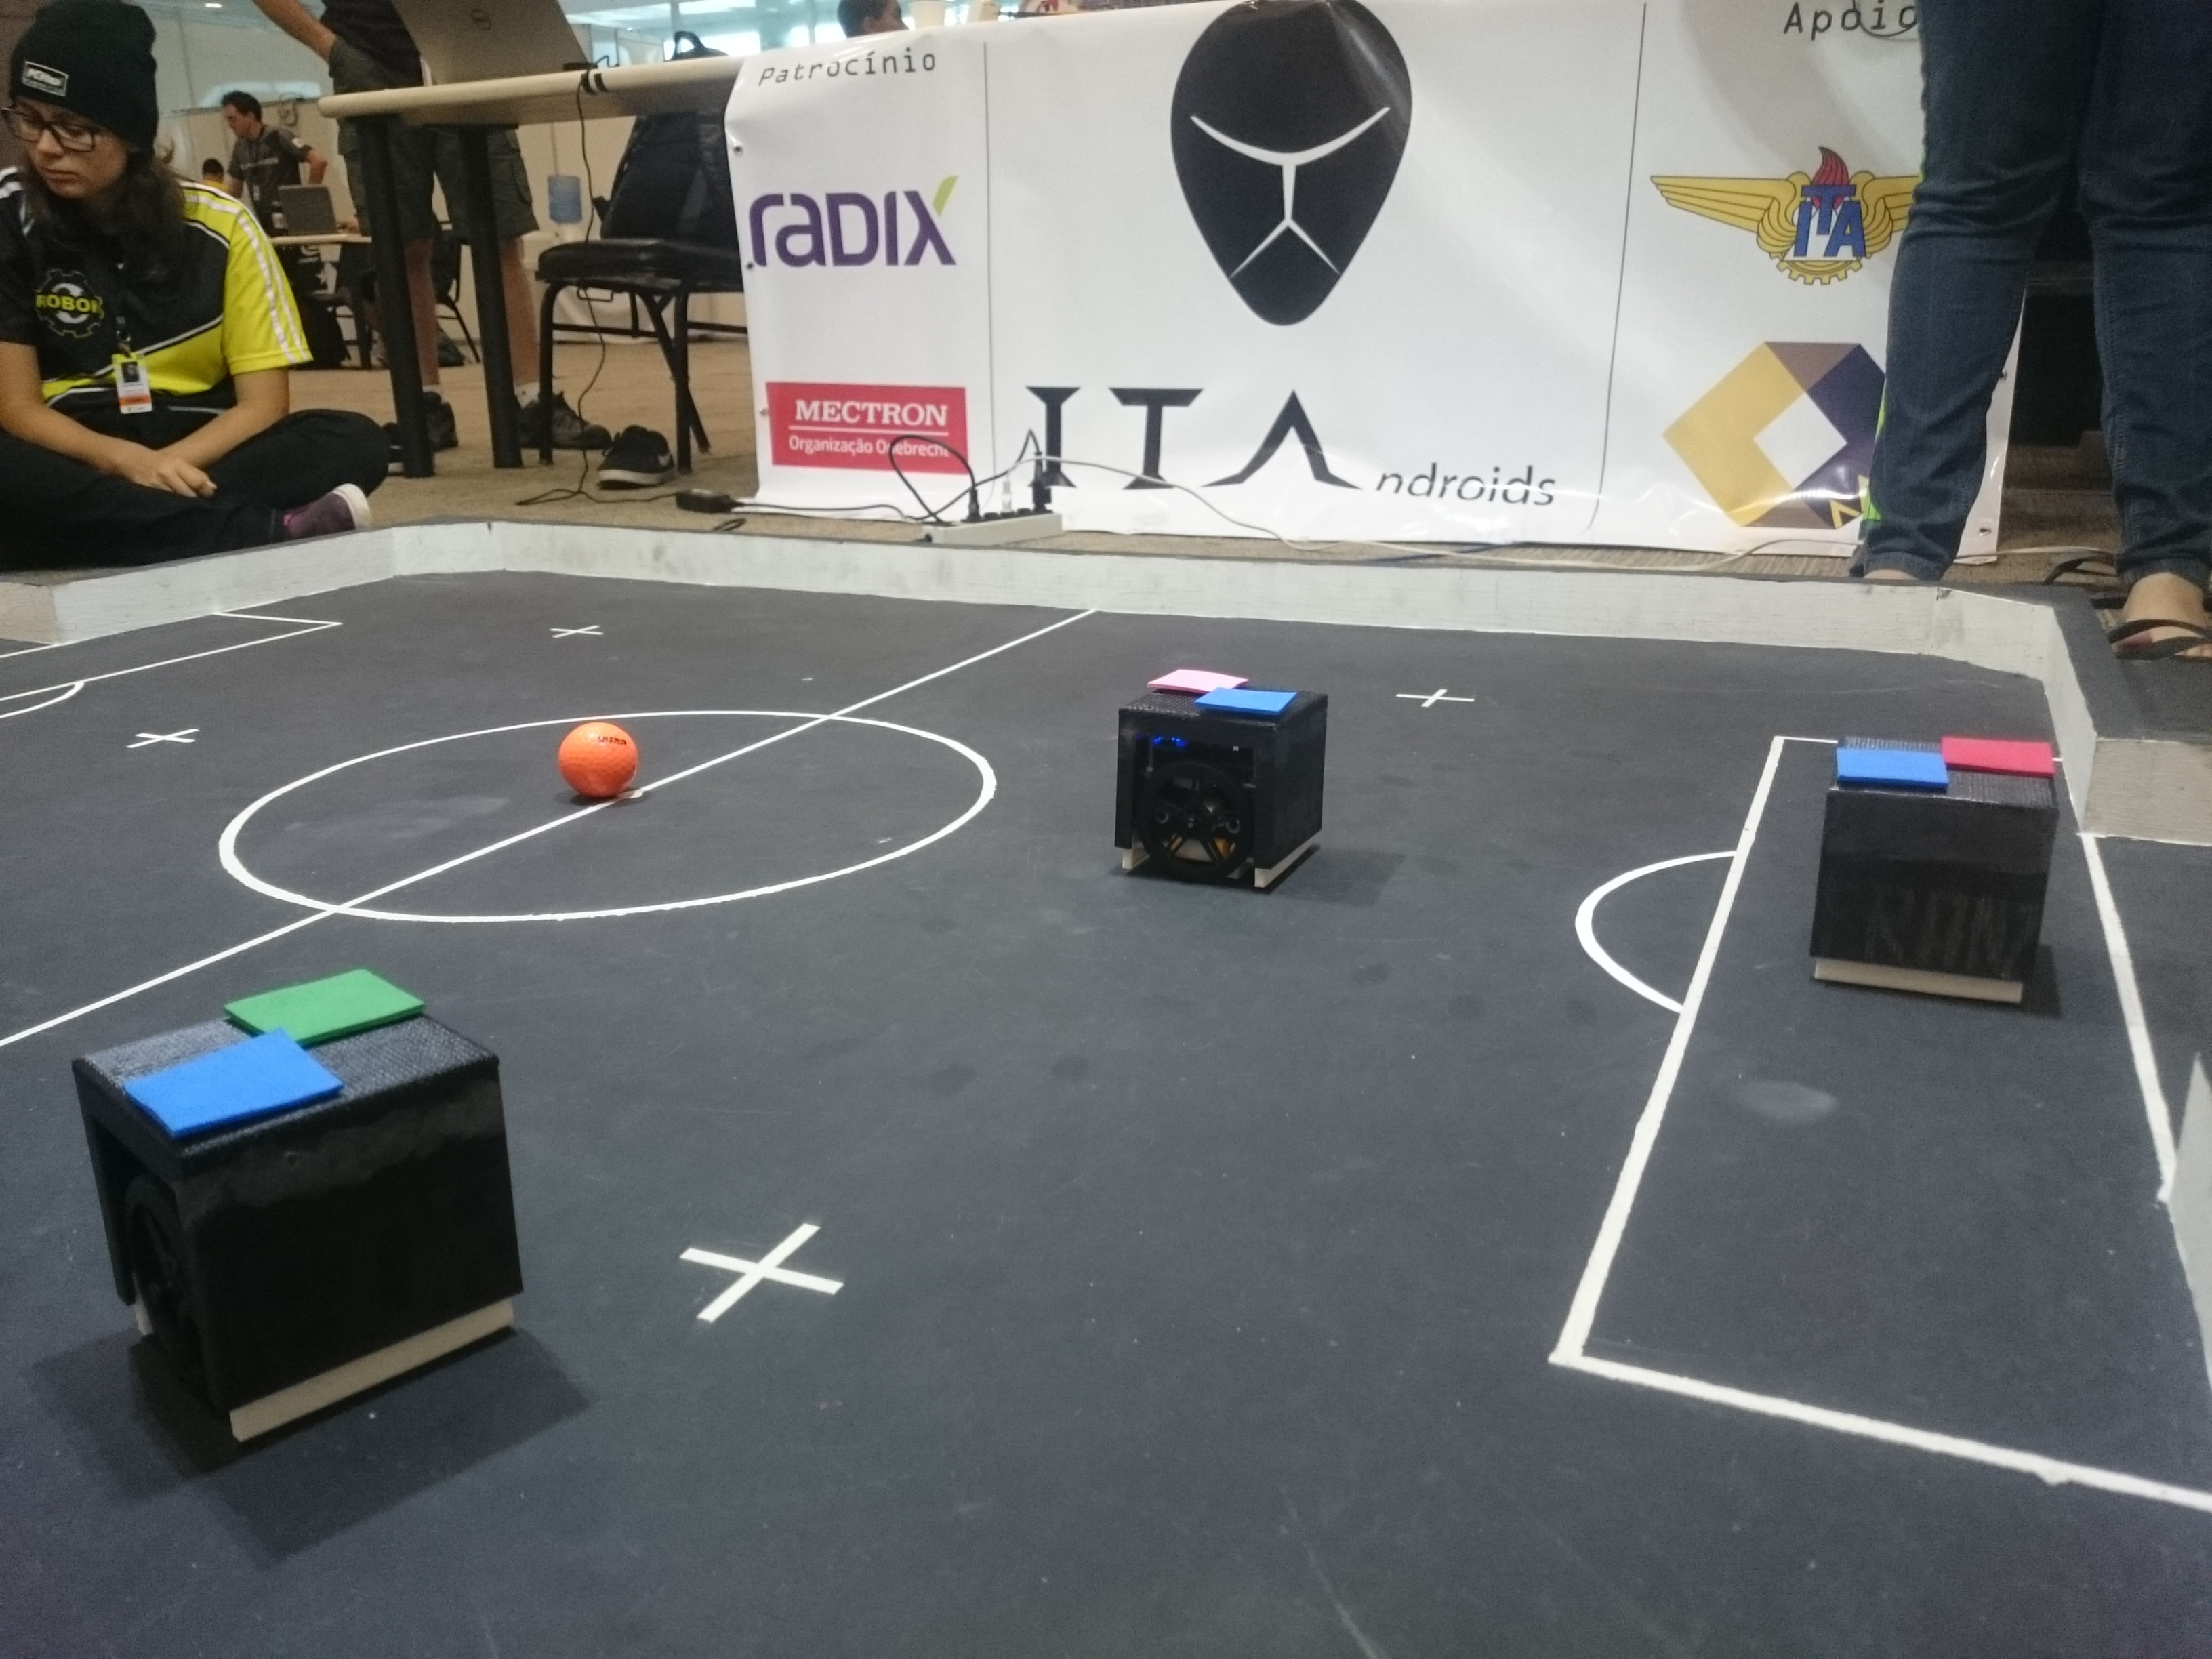
\includegraphics[width=0.5\textwidth]{figures/vss-min.JPG}
   \caption{ITAndroids Robots of the IEEE VSSS category.} \label{fig:vss}
\end{figure}


The Figure \ref{fig:vss} shows the robots used in competitions. The computational vision used by the ITAndroids team can be found in more detail in \cite{zickler2009ssl} and uses a camera at the top of the field that passes information to a computer processing, as seen in Figure \ref{fig:funcioamento}.

\begin{figure}[H]
	\centering
		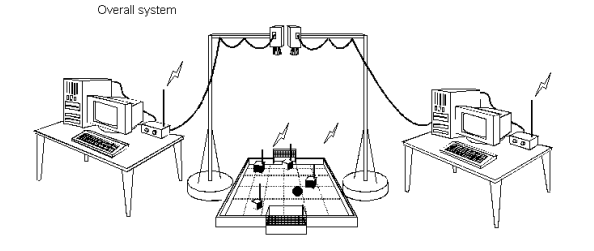
\includegraphics[width=0.7\textwidth]{figures/overview.png}
  \caption{Representation of the technical functioning of a VSS game.}
	\label{fig:funcioamento}
\end{figure}

Each robot was designed with two side wheels and two free balls at the front and back to maintain balance. This characteristic makes it a differential robot. That is, we have control over linear and angular speeds, but it is not possible to move the robot sideways. The language used for the project was C ++ because it is a language that has a high execution speed and has good scalability for a large project.

In this context, several issues arise to be solved in order to have a winning team. In this project, the following strategy problem will be addressed: given the position and speed of each robot and ball, one must choose which position a particular robot will go with, which controller and which path planning to use. One must also put together a plan for future actions, planning a sequence of positions that the robot must go to to make a goal.

The strategy algorithm should run at run time of at most 10 ms for the entire team, which is the camera sampling time discounted from computational view processing time. Most of this time is spent on the trajectory planning used, which is the Rapidly-exploring Random Tree (RRT). The time for each execution of an RRT is 1 ms, according to \cite{franzoni_rrt}, limiting it around a limit of twelve algorithm calls by completing the strategy, with a margin of error of thirty-three percent . The importance of not exceeding this maximum time is emphasized, since if this happens an image of the camera is lost and the operation of the game is carried out in a delayed way.

A dynamic positioning scheme must therefore be set up in which there is no fixed attacker, defender or goalkeeper, but rather that the positions depend on and adapt to the playing position, ensuring that the three players can be better positioned and free to choose their next actions. This must be done because the fixed positioning scheme does not work very well in the context of the Very Small Size category, since it greatly limits the offensive and defensive capacity of the team.

To solve this problem, it was chosen as the main algorithm for decision making the Behavior Tree. This algorithm was chosen from among options such as Finite State Machine and Decision Tree. An introduction to these issues can be found in \cite{orozcomaquinas} for finite state machine and \cite{decision_tree} for Decision Tree. The choice is based on the decision of a reference team in world robot football, the Near East University team: the NEUIslanders, as described in \cite{NEUIslanders_ssl}.

This work brings as a contribution the implementation of the Behavior Tree method for the Very Small Size category, being the first scientific publication of this subject in the literature.

\subsection{Behavior Tree}

To build a Behavior Tree (BT), you must first understand the basics of its structure. A BT is a Tree in the sense given by graph theory, as explained in \cite{west2001introduction}. By definition, each node of this tree is called behavior.

The nodes of a Behavior Tree are differentiated into two types: the leaf nodes, which are the nodes of the tree that has no children and the compound nodes, which may have one or more children.

All nodes return, at the end of their execution, one of the following three states: TRUE, FALSE, or RUNNING, to indicate, respectively, that the node was successfully terminated, that it was terminated without success, or that the algorithm should execute that node for at least one more iteration.

\subsubsection{Leaf Nodes}

The leaf nodes are the terminal nodes of the Tree and they represent the lowest and most concrete actions of the strategy. They are divided into two types: action nodes and conditional nodes.

\textbf{Action nodes:} These are nodes that actually perform an action, such as moving to the ball.

\textbf{Conditional nodes:} These are nodes that only return a state without performing any concrete action, such as checking if the team is attacking. They are used to control which nodes will be run in conjunction with the compound nodes.

\subsubsection{Composite Nodes}

Compound nodes are tree nodes, which are responsible for choosing which nodes to run. They are completely reusable in the sense that only one implementation of each type of compound node must exist and it can be used in several parts of the code. The main types of these nodes that were used for the strategy are listed below:

\textbf{Selector Behavior:} In this behavior, one of your children is selected to be accessed next. It is used when you have several ways to perform the same action and one should choose the best one in a given situation. It works by running the children in a certain order, and as soon as one of the children returns TRUE or RUNNING, that node returns the same value. If a child returns FALSE, the next child will be executed. If no child succeeds or returns to be executed again, the node returns FALSE.

\textbf{Sequence Behavior:} This node executes each of its children in a well-defined and fixed sequence. It is used to do sequenced actions to complete a larger goal, for example: kicking the ball to the opponent's goal requires that the allied robot is behind the ball, which means that getting behind the ball and then kicking the ball represent sequenced actions. It works so that when a child returns RUNNING or FALSE, the behavior returns the same value, and when a child returns TRUE, it advances to the next child. If all children return TRUE, the behavior succeeds and also returns TRUE.


\textbf{Parallel Behavior} The purpose of this node is to execute all its children at the same time, a fact that can be obtained when using parallel processing or not. In the implementation of this work the non-parallel version of the algorithm was used. If a child returns FALSE, the behavior returns FALSE. If all children return TRUE, the behavior returns TRUE. In all other situations, the behavior returns RUNNING and continues its execution by at least one other iteration.

\textbf{Decorator:} The name for this behavior is inspired by the Decorator concept in Software Design Pattern, which can be studied in \ cite {hunt2013gang}. In the Behavior Tree context, this node has only one child and it modifies the behavior of the child in some way. A decorator can be several types, but the most used in the project were:

\begin{enumerate}
\item AlwaysFail and AlwaysSucceed: which cause the child to always return FALSE or always return TRUE respectively.
\item UntilFail and UntilSucceed: cause the fiho to always return RUNNING unless it returns FALSE or TRUE, respectively.
\item Invert: Changes the child's return from FALSE to TRUE and TRUE to FALSE.
\end {enumerate}

\subsection{Technician}

A Behavior Tree, although it can easily model complex behaviors, is not always the best choice for certain situations. Therefore, the strategy was divided into levels of different abstractions, in which a Technician, represented by the Coach class, would be responsible for choosing and administering which tree each of the three players should use at the moment.
With this implementation, we have an external agent controlling the players' function by choosing a BT, which can be a tree for a goalkeeper, a principal and an assistant. This means that at any given time, the coach can choose to have the team have 1 goalkeeper, 1 main and 1 assistant to even 3 main ones at the same time. The expected requirements for each of these roles will be discussed below. In addition, it is also the role of the coach to choose the role of each player at each iteration of the code, so that the positions of the players are not fixed during the course of the game.

\section{Results and Discussion}

Os resultados a seguir foram obtidos estudando o comportamentos de equipes adversárias na competição, além de diversos testes com o time de robôs da ITAndroids contra si mesmo em simulações computacionais em um simulador feito pela própria equipe, como mostrado na Figura \ref{fig:simulator}.

\begin{figure}[H]
	\centering
	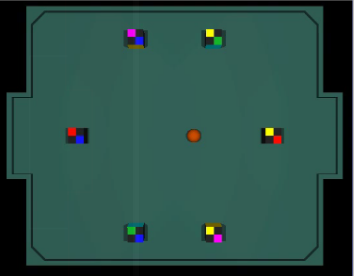
\includegraphics[width=0.6\textwidth]{figures/SimulatorWithoutButtons.png}
	\caption{Simulador da ITAndroids.}
	\label{fig:simulator}
\end{figure}

\subsection{Goleiro}

O goleiro é o jogador que deve ficar próximo ao gol aliado com o objetivo de proteger o gol de ataques oponentes. 
A BT criada para o goleiro está representada na Figura \ref{fig:goalier_bt}.

\begin{figure}[H]
	\centering
	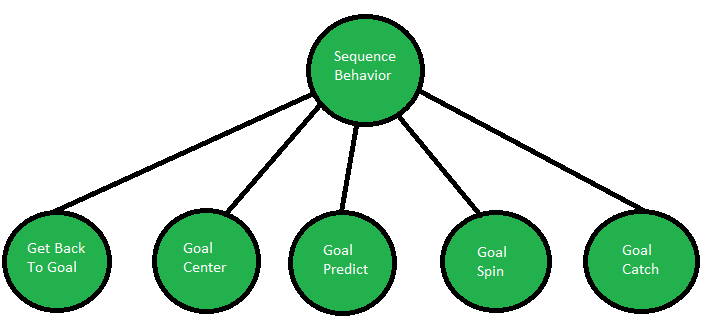
\includegraphics[width=0.8\textwidth]{figures/Goalier_BT.png}
   	\caption{Behavior Tree para o goleiro.} \label{fig:goalier_bt}
\end{figure}

Como visto, ela é composta por um nó do tipo Sequence Behavior, que irá executar os seus filhos em sequência. Esse papel, então, executa as seguintes ações prioritando as primeiras a aparecerem na seguinte lista:

\begin{itemize}

\item \textbf{Get Back to Goal Behavior} Volta para o gol, caso que, se por algum motivo ele esteja fora do próprio.

\item \textbf{Goal Center} Fica centralizado no gol quando a bola estiver longe, de forma que o jogador possa rapidamente ir para qualquer um dos lados quando a bola se aproximar.

\item \textbf{Goal Predict} Prediz para onde a bola irá quando ela estiver rápida e longe do gol.

\item \textbf{Goal Spin} Gira quando está perto da bola e não tem oponente perto da bola para jogá-la para longe.

\item \textbf{Goal Catch} Comportamento que o goleiro deverá fazer quando não fizer nenhum outro, por isso sua última posição na sequência. Ele acompanha o movimento da bola com o goleiro sobre a linha do gol.

\end{itemize}



\subsection{Principal}

O jogador com o papel de Principal é o jogador mais ativo do time, que deve estar constantemente avançando em direção a bola. Esse papel e o goleiro são as únicas posições que efetivamente deverão tocar na bola. A árvore \ref{fig:principal_bt} foi desenvolvida para o principal, sendo a árvore mais complexa dentre os papéis.

\begin{figure}[H]
	\centering
	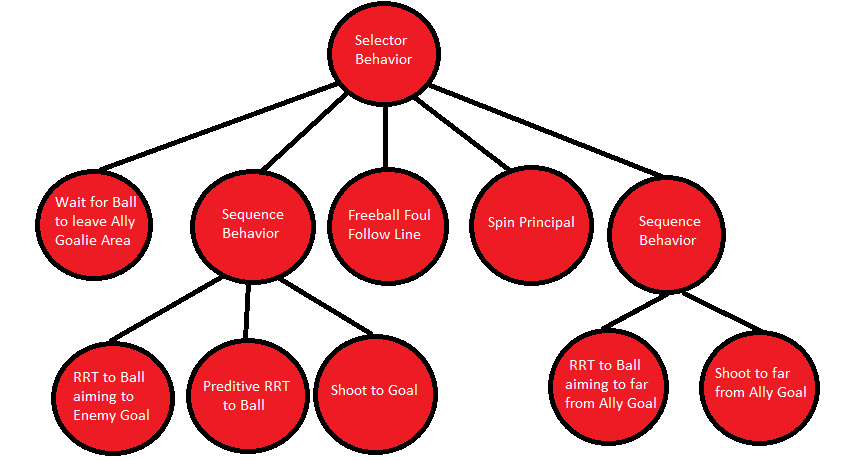
\includegraphics[width=0.8\textwidth]{figures/Principal_BT.png}
   	\caption{Behavior Tree para o principal.} \label{fig:principal_bt}
\end{figure}   

Conforme a Figura \ref{fig:principal_bt}, a raiz da árvore do principal é um Selector Behavior que escolhe uma das ações a ser realizada. Essa BT tem mais dois outros nós compostos, que são dois Sequence Behavior usados para o posicionamento atrás da bola, seguido pelo chute. Uma descrição dos nós folha utilizados se encontra abaixo:

\begin{itemize}

\item \textbf{Wait for Ball to leave Ally Goalie Area} Esse Behavior utiliza a Triangução de Delaunay. Esse comportamento deve evitar que o jogador entre na área do goleiro para não sofrer penâlti, conforme descrito na Figura \ref{fig:penalty}. O jogador se pocionará de acordo com posições escolhidas pelo usuário, calibradas com um arquivo de configuração .txt.

\begin{figure}[H]
	\centering
	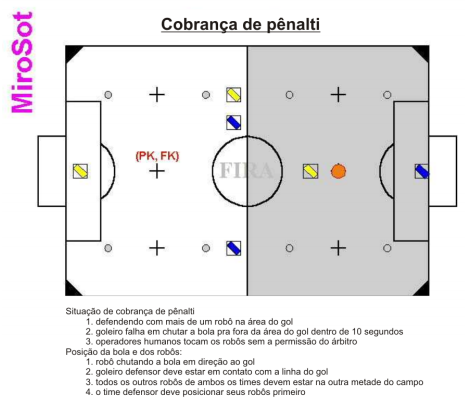
\includegraphics[width=0.7\textwidth]{figures/campo_penalty.png}
   \caption{Descrição da penalidade pênalti.} \label{fig:penalty}
\end{figure}

\item \textbf{RRT to Ball aiming to Enemy Goal} Irá usar o algoritmo de planejamento de trajetórias RRT para se deslocar atrás da bola com direção apontando para o gol oponente. Usado para se aproximar da bola e, em seguida, trocar para o próximo behavior, o Predictive RRT to Ball.

\item \textbf{Predictive RRT to Ball} Usa uma predição linear considerando que a bola continuará na mesma velocidade. Usado para se chegar na bola com mais precisão quando próximo a ela. Chega atrás da bola mirando para o gol.

\item \textbf{Shoot to Goal} Esse behavior só é chamado quando o jogador já está alinhado com a bola e o gol oponente. Esse comportamento acelera rapidamente o robô em linha reta para chegar no gol com uma velocidade alta.

\item \textbf{Free Ball Foul Follow Line} Esse behavior é um específico para situações de falta do tipo Bola Livre, conforme descrito na Figura \ref{fig:bola_livre}. Quando for detectado uma dessas posições, o jogador deve acelerar o mais rápido possível em direção à bola para ter o controle dela antes do oponente.

\begin{figure}[H]
	\centering
	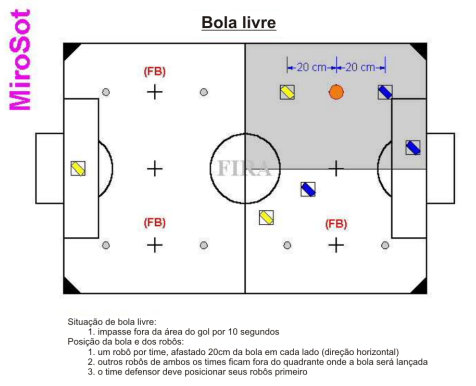
\includegraphics[width=0.7\textwidth]{figures/bola_livre.png}
   \caption{Descrição da penalidade bola livre.} \label{fig:bola_livre}
\end{figure}

\item \textbf{Spin Principal} Esse nó deve ser chamado quando a bola estiver em um dos quatros campos do campo. Caso seja um campo defensivo, o jogador irá girar para jogar a bola para frente; caso seja um na zona de ataque, o jogador girará para por a bola no centro do campo e continuar o ataque.

\item \textbf{RRT to Ball aiming to far from Ally Goal} Irá usar o algoritmo de planejamento de trajetórias RRT para se deslocar atrás da bola com direção apontando para a zona de ataque (longe do gol aliado). Usado para se aproximar da bola e se posicionar para, em seguida, chamar o Behavior Shoot to Far from Ally Goal.

\item \textbf{Shoot to Far from Ally Goal} Esse behavior só é chamado quando o jogador já está alinhado com a bola e o para frente (para longe do gol aliado). Esse comportamento acelera rapidamente o robô em linha reta para pôr a bola na zona de ataque.

\end{itemize}


\subsection{Auxiliar}

	O auxiliar é um papel que tem apenas uma função: posicionar-se da melhor forma possível para manter um ataque consistente. A ideia é que, caso a situação seja oportuna, o auxiliar se torne o principal e comece a atacar a bola. Para escolher a posição que o auxiliar deverá ficar em uma determinada situação de jogo, foi utilizado a Triangulação de \cite{delaunay34} sobre o grafo de \cite{voronoi08}. Esse algoritmo foi aplicado similarmente a \cite{akiyama2007multi}, relativo também à futebol de robôs.

	A Behavior Tree do auxiliar, por sua vez, é muito simples, representada por apenas um nó que tem como função se posicionar em lugar ótimo. Sua árvore, é representada simplesmente pela Figura \ref{fig:auxiliar_bt}.

\begin{figure}[H]
	\centering
	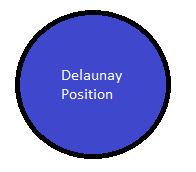
\includegraphics[width=0.3\textwidth]{figures/Auxiliar_BT.png}
   \caption{Behavior Tree para o auxiliar.} \label{fig:auxiliar_bt}
\end{figure}


\section{Conclusion}
	In this article, an implementation of the Behavior Tree method for the category of robots of Very Small Size Soccer was presented, which was briefly described its operation. We have shown the paper scheme used as well as the Behavior Tree implemented for each of them, as well as a detailed description of all the tree nodes.

The Scientific Initiation Project presented good results, especially with respect to the ITA team's victory until the quarterfinals of CBR 2017, yielding the seventh place to the team among more than 25 participating teams. In addition to the fact that ITAndroids won the first place in the national competition of VSSS Turing Cup 2017, which occurred in late September 2017.

From a technical point of view, the use of the Behavior Tree algorithm, already consecrated and used by world-class teams, proved to be feasible and functional in real matches of competitions. However, problems such as low scalability and low reusability were shown in the developed strategy. This means that changes still have to be made in BT, especially regarding the use of more parallel-type nodes to remove these problems.

\begin{thebibliography}{00}
\bibitem{decision_tree} Russel, S. and Norvig, P., 2009. Artificial Intelligence: A Modern Approach, Prentice Hall, Vol. 3, pp. 697–707. 3rd edition

\bibitem{zickler2009ssl} Zickler, S., Laue, T., Birbach, O., Wongphati, M. and Veloso, M., 2009. “Ssl-vision: The shared vision system for the
robocup small size league”. In Robot Soccer World Cup. Springer, pp. 425–436.

\bibitem{CBR2008} CBR, 2008. \url{Http://www.cbrobotica. org/wp-content/uploads/2014/03/VerySmall2008_en.pdf}.

\bibitem{orozcomaquinas} Coelho, M.M.A., 2016. “Máquinas de estados finitos”.

\bibitem{franzoni_rrt} Okuyama, I.F., 2017. TRAJECTORY PLANNING CONSIDERING ACCELERATION LIMITS FOR AN AUTONOMOUS SOCCER PLAYER. Trabalho de graduação, Instituto Tecnológico de Aeronáutica.

\bibitem{west2001introduction} West, D.B. et al., 2001. Introduction to graph theory, Vol. 2. Prentice hall Upper Saddle River.

\bibitem{delaunay34} Delaunay, B., 1934. “Sur la sphére vide”. Bulletin de l’Académie des Sciences de l’URSS, Vol. 6, pp. 793–800.

\bibitem{voronoi08} Voronoi, G., 1908. “Nouvelles applications des paramètres continus à la théorie des formes quadratiques”. Journal fürdie Reine und Angewandte Mathematik, Vol. 133, pp. 97–178.

\bibitem{NEUIslanders_ssl} Abiyev, R.H., Şenol Bektas, Akkaya, N. and Aytac, E., 2017. “Neuislanders 2017 team description paper”. Robocup.

\bibitem{hunt2013gang} Hunt, J., 2013. “Gang of four design patterns”. In Scala Design Patterns, Springer, pp. 135–136.

\bibitem{akiyama2007multi} Akiyama, H. and Noda, I., 2007. “Multi-agent positioning mechanism in the dynamic environment”. In Robot Soccer World Cup. Springer, pp. 377–384.

\end{thebibliography}

\end{document}
